\documentclass[11pt,letterpaper]{article}

\usepackage{fancyhdr}
\usepackage[latin1]{inputenc}
\usepackage{amsmath}
\usepackage{amsfonts}
\usepackage{amssymb}
\usepackage{graphicx}
\usepackage[hmargin=2cm,vmargin=2.5cm]{geometry}
\usepackage[normalem]{ulem}
\usepackage{enumerate}
\usepackage{hyperref}
\usepackage{palatino}
\usepackage{graphics}

\newcommand{\workingDate}{\textsc{November 2018}}
\newcommand{\courseName}{MTH 201}
\newcommand{\institution}{Grand Valley State University}

\newenvironment{problem}[2][Problem]{\begin{trivlist}
\item[\hskip \labelsep {\bfseries #1}\hskip \labelsep {\bfseries #2.}]}{\end{trivlist}}

\pagestyle{fancy}
\setlength\parindent{0in}
\setlength\parskip{0.1in}
\setlength\headheight{15pt}

%%%%%%%%%%% HEADER / FOOTER %%%%%%%%%%%
\rhead{R. Talbert}
\chead{\textsc{Lab 7}}
\lhead{\textsc{\courseName}}

\begin{document}

\begin{flushright}
	\begin{Large}
		Lab 7: Applied optimization
	\end{Large}
\end{flushright}

\noindent
\textbf{Overview:} In this lab, get further practice with applied optimization and have computer tools to help you srt up and analyze optimization problems. 



\subsection*{Instructions}

In the Lab Tasks section below, there are three problems asking you to find the optimum value of something. Choose \emph{exactly one} of these and give a complete, clear, and correct solution. 

In order to earn a Satisfactory grade on this lab, your writeup must: 
\begin{itemize}
    \item Begin by clearly indicating which one of the three problems you are solving. 
    \item Arrive at a correct answer. 
    \item Show all relevant work that leads to the answer. In particular, \emph{your work must include an explanation of why your answer is truly the maximum or minimum value of the quantity you are optimizing. Simply finding a critical number without testing it, will result in an Unsatisfactory grade and you'll have to revise it to fill in the details}. 
    \item Be clearly written and include English explanations of what you are doing. \emph{Writeups that are just computations with minimal or no explanations will be graded Unsatisfactory and will need to be revised.} 
    \item Clearly state all the variables involved in the solution, both the notation being used for the variable as well as a statement of what the variable stands for and the units of measurement being used. 
    \item Be neatly typewritten. No handwritten work is accepted except for diagrams, and you should try to computer-draw those first before hand-drawing them. 
\end{itemize}

\emph{Special note:} For this lab, you may use a computer to do any mathematical computation you need to do, including taking derivatives or solving equations. If you use a web-based tool like Wolfram Alpha or Desmos, please include links to all your computer work. For example if you use WA to take the derivative of $x^2$, give a link like this: \url{https://www.wolframalpha.com/input/?i=derivative+of+x%5E2} 

You must include a link to your work if you do work on a website, otherwise it will count as insufficient work shown, and you'll be asked to revise it. 

Similarly if you use an offline computer program to do any math work, include a printout or screenshot of the work you did and the details of what tool you used. 


\subsection*{Lab tasks}

Remember: \emph{Do just one (1) of the following.} 

\begin{problem}{1}
Suppose that 600 meters of fence are use to enclose an animal pen that is shaped like a rectangle with a semicircular end. (See the picture below.) Find the dimensions of the pen that gives the maximum possible area. Note that in the diagram, the dotted line is not part of the pen, and there is no fence there; it merely indicates where the rectangle stops and the semicircle begins. 
\begin{center}
    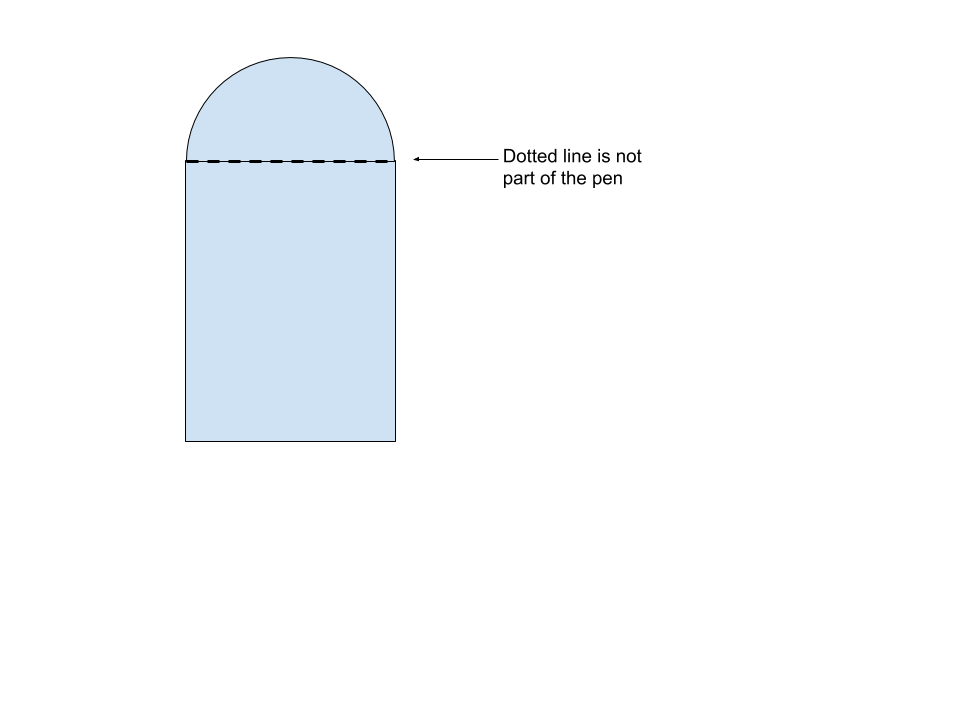
\includegraphics[width=4in]{l7p1.png}
\end{center}


\end{problem}

\begin{problem}{2}
A new apartment complex is being built near GVSU (because you know we don't have enough of these already) with 100 units being available. The managers are trying to figure out what rent to charge, in order to maximize their profits. When they charge \$900 per month, all 100 of the units will be rented, and one unit will become vacant for every \$10 increase in rent. Furthermore, the managers have to spend money for maintenance of the units --- the maintenance cost is \$100 per month for each unit that is occupied. (Assume vacant units cost nothing to maintain.) 
\begin{enumerate}
    \item Find a formula for the number of units occupied per month, as a function of the amount of rent being charged. (To begin, let $r$ be the monthly rent and see if you can determine the number of units occupied for various specific values of $r$. Then try to make a formula for any value of $r$.) 
    \item Find a formula for the net cash intake (revenue minus maintenance cost) and determine the rent amount $r$ that will maximize this cash intake. 
\end{enumerate}
\end{problem}

\begin{problem}{3} Alice can swim 3 miles per hour and run at 8 miles per hour. She is standing one bank of a river that is 300 feet wide and wants to reach a point located 200 feet downstream on the other side as quickly as possible. She will swim diagonally across the river and then jog along the river bank. What route is best for Janice? 

\end{problem}

\end{document}